\documentclass[12pt,letterpaper]{report}
\usepackage[margin=1in]{geometry}
\usepackage{graphicx}
\usepackage{amsmath}
\usepackage[font=small,labelfont=bf]{caption}
\usepackage[justification=centering]{caption}
\usepackage{tikz}
\usepackage{circuitikz}
\usepackage{siunitx}
\usepackage{float}
\newlength \figwidth
\setlength \figwidth {0.75\linewidth}

\begin{document}

\title{E153 Laboratory Assignment \#6}
\author{Courtney Keeler and Stephen Pinto\\
Harvey Mudd College}
\date{November 20, 2013}
\maketitle

\section*{List of Materials}
\begin{itemize}
	\item Tektronix 2212 Oscilloscope
	\item Pomona 4550B (10X probe)
	\item Elenco LCM-1950 Multimeter
	\item 2N3904 transistor x2
	\item Standard resistors
	\item Standard capacitors
\end{itemize}

\section*{Purpose}
The purpose of this lab is to build a pre-designed common emitter amplifier and compare the actual performance to the simulated performance. The purpose is also to examine the effects of loading on the CE amplifier circuit by cascading the amplifier with a simple emitter follower.

\section*{Common Emitter Amplifier}
\begin{figure}[H]
\centering
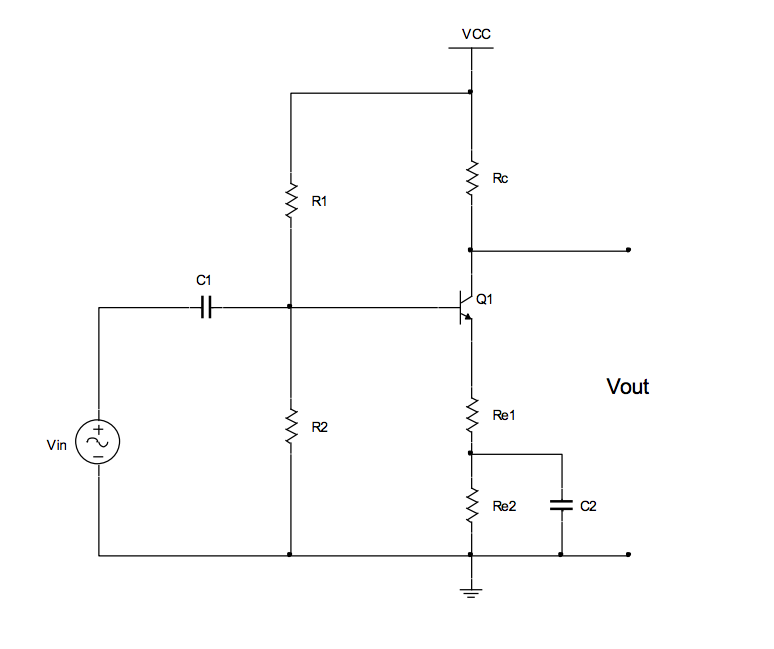
\includegraphics[width=\figwidth, keepaspectratio=true]{lab6_images/cea.png}
\caption{Common Emitter Amplifier. Image from Design Exercise 1.}
\label{fig:cea}
\end{figure}

\subsection*{Procedure}

\begin{enumerate}
\item Measure the actual component values used in the CEA design (shown in Figure \ref{fig:cea})
\item Recalculate the gain and frequency response of the CEA with the values from the previous step
\item Build the common emitter transistor amplifier designed in design project \#1
\item Compare the actual gain and frequency response values with the simulated values
\item Tweak component values 
\end{enumerate}

\subsection*{Results}

Measured component values for common emitter amplifier:
\begin{itemize}
\item $R_C$ = 17.67 k$\Omega$
\item $R_1$ = 10.1 M$\Omega$
\item $R_2$ = 18.24 M$\Omega$
\item $R_{E1}$ = 550 $\Omega$
\item $R_{E2}$ = 4.58 k$\Omega$
\item $C_1$ = .339 + .342 = .681 $\mu$F
\item $C_2$ = 323.5 + 332.3 = 655.8 $\mu$F
\item $\beta$ = 231
\end{itemize}

%photo 297
%gain is 26.6

%when both emitter resistors are bypassed, the gain beccomes just over 200

\subsection*{Calculations}

%real resistor and capacitor values
We want to recalculate the expected gain using the actual component values:
$$
A_v = \frac{-\beta R_C}{r_{\pi}+(1+\beta)R_{E1}}.
$$
First we must calculate $I_B$ so that we can know the value of $r_{\pi}$:
$$
I_B = \frac{V_{th}-0.7}{R_{th}+(1+\beta)(R_{E1}+R_{E2})},
$$
where
$$
V_{th} = \frac{R_2}{R_1+R_2}V_{cc} = 12.87 \text{ V}\, \text{ and } \, 
R_{th} = R_1||R_2 = 6.5 \text{ M}\Omega.
$$
We can plug all of this in to find:
$$
A_v = -28.34.
$$

\subsection*{Physical Implementation \& Analysis}

\begin{figure}[H]
\centering
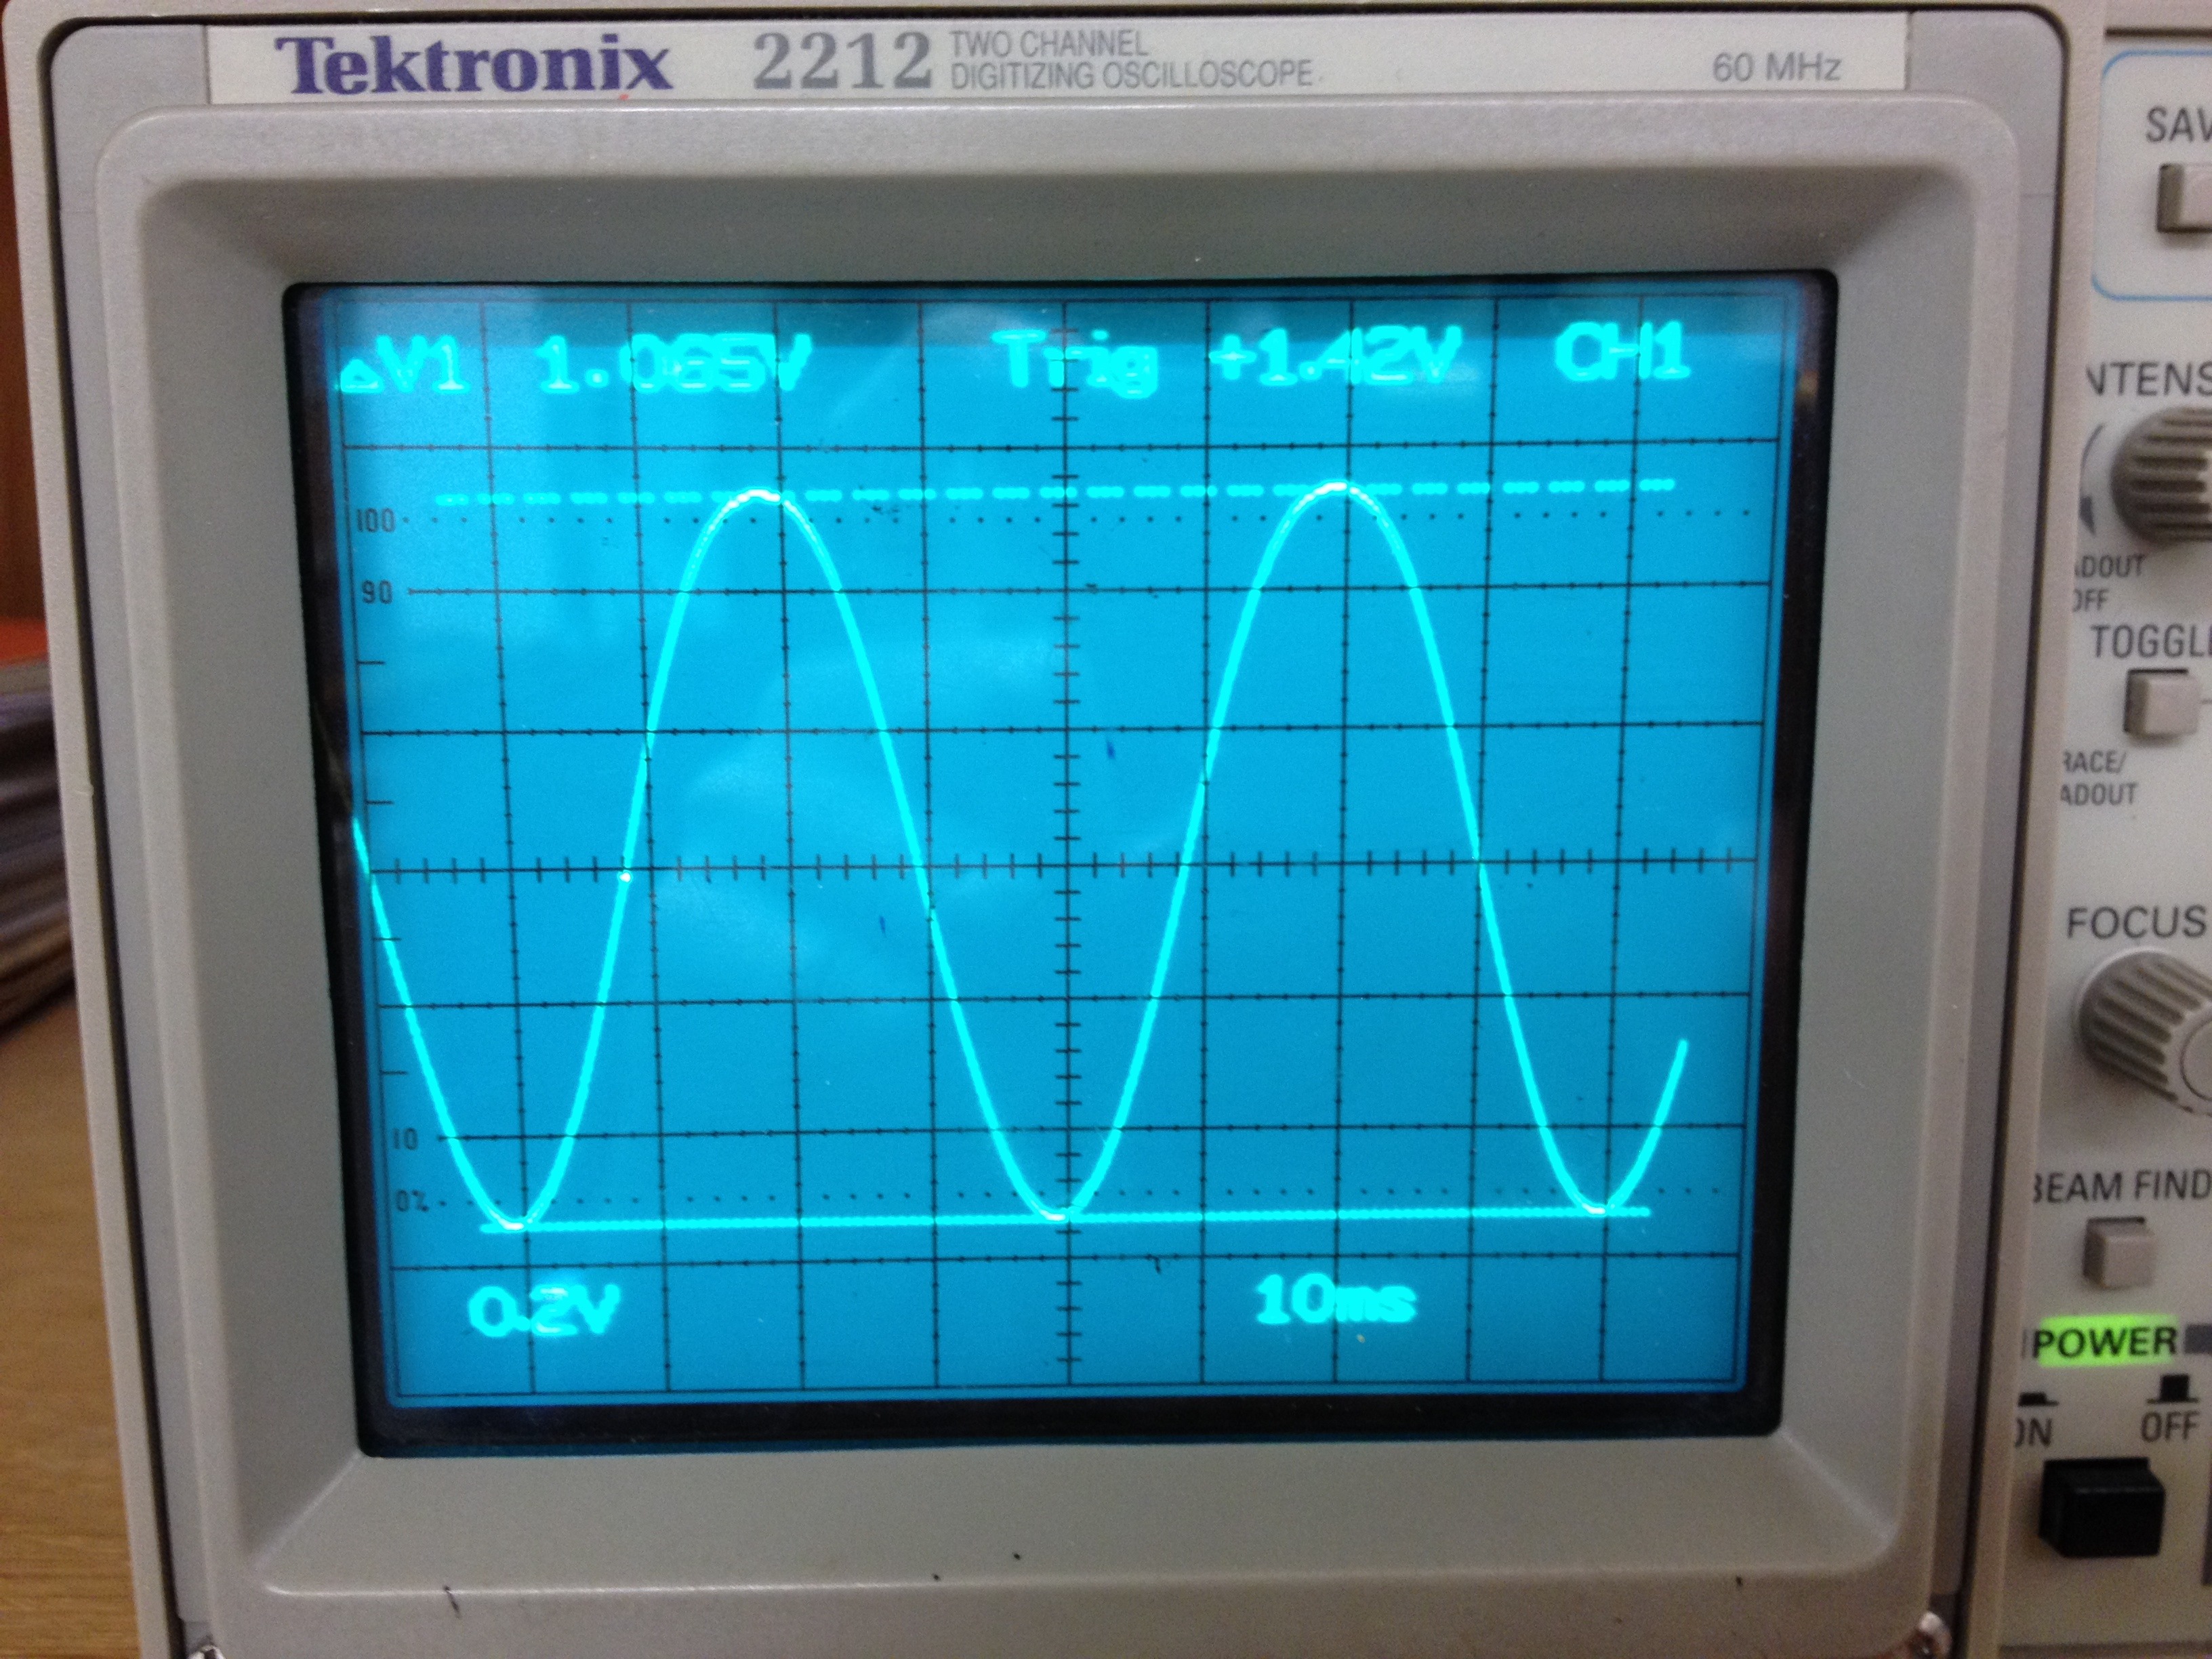
\includegraphics[width=\figwidth, keepaspectratio=true]{lab6_images/simple_output.jpg}
\caption{Output from Common Emitter Amplifier with input of 400  $mV_{pp}$.}
\label{fig:simple_output}
\end{figure}

Figure \ref{fig:simple_output} shows the 10.65 $V_{pp}$ output from the common emitter amplifier with an input of 400 $mV_{pp}$ - making the actual gain -27. While the magnitude of this measured gain is 6\% lower than expected, at least the measured gain is within the design specifications of $-25 \pm 10\%$. The reasons for this discrepancy could be 

\section*{Emitter Follower}

\begin{figure}[H]
\centering
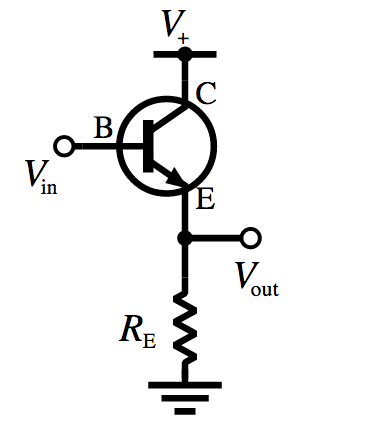
\includegraphics[width=0.2\linewidth, keepaspectratio=true]{lab6_images/emitter_follower.png}
\caption{Basic Emitter follower. Image from Wikipedia.}
\label{fig:emitter_follower}
\end{figure}

\subsection*{Procedure}

\begin{enumerate}
\item Add a simple emitter follower (shown in Figure \ref{fig:emitter_follower}) to the CE amplifier from the previous section
\item Calculate the theoretical voltage gain reduction caused by the added loading
\item Measure the actual voltage gain
\end{enumerate}

\subsection*{Calculations}

Without the emitter follower attached, the output amplitude, as shown in Figure \ref{fig:simple_output}, is 10.65 $V_{pp}$. Since the emitter follower has some non-infinite input impedance, the output signal from the common emitter amplifier should have a reduced amplitude due to loading. This expected reduction is summarized by the following (where CEA stands for Common Emitter Amplifier and EF for Emitter Follower)
$$
V_{CEA,closed} = V_{CEA,open}\frac{R_{in,EF}}{R_{out,CEA}+R_{in,EF}},
$$
where $R_{in,EF}$ is approximately $(1+\beta)R_E$ since $r_{\pi,EF} \ll (1+\beta)R_E$ and $R_{out,CEA} = R_C$ . Thus
$$
V_{CEA,closed} = 10.65 \frac{(1+243)982}{17670+(1+243)982} = 9.87 V.
$$


\subsection*{Results}

\begin{figure}[H]
\centering
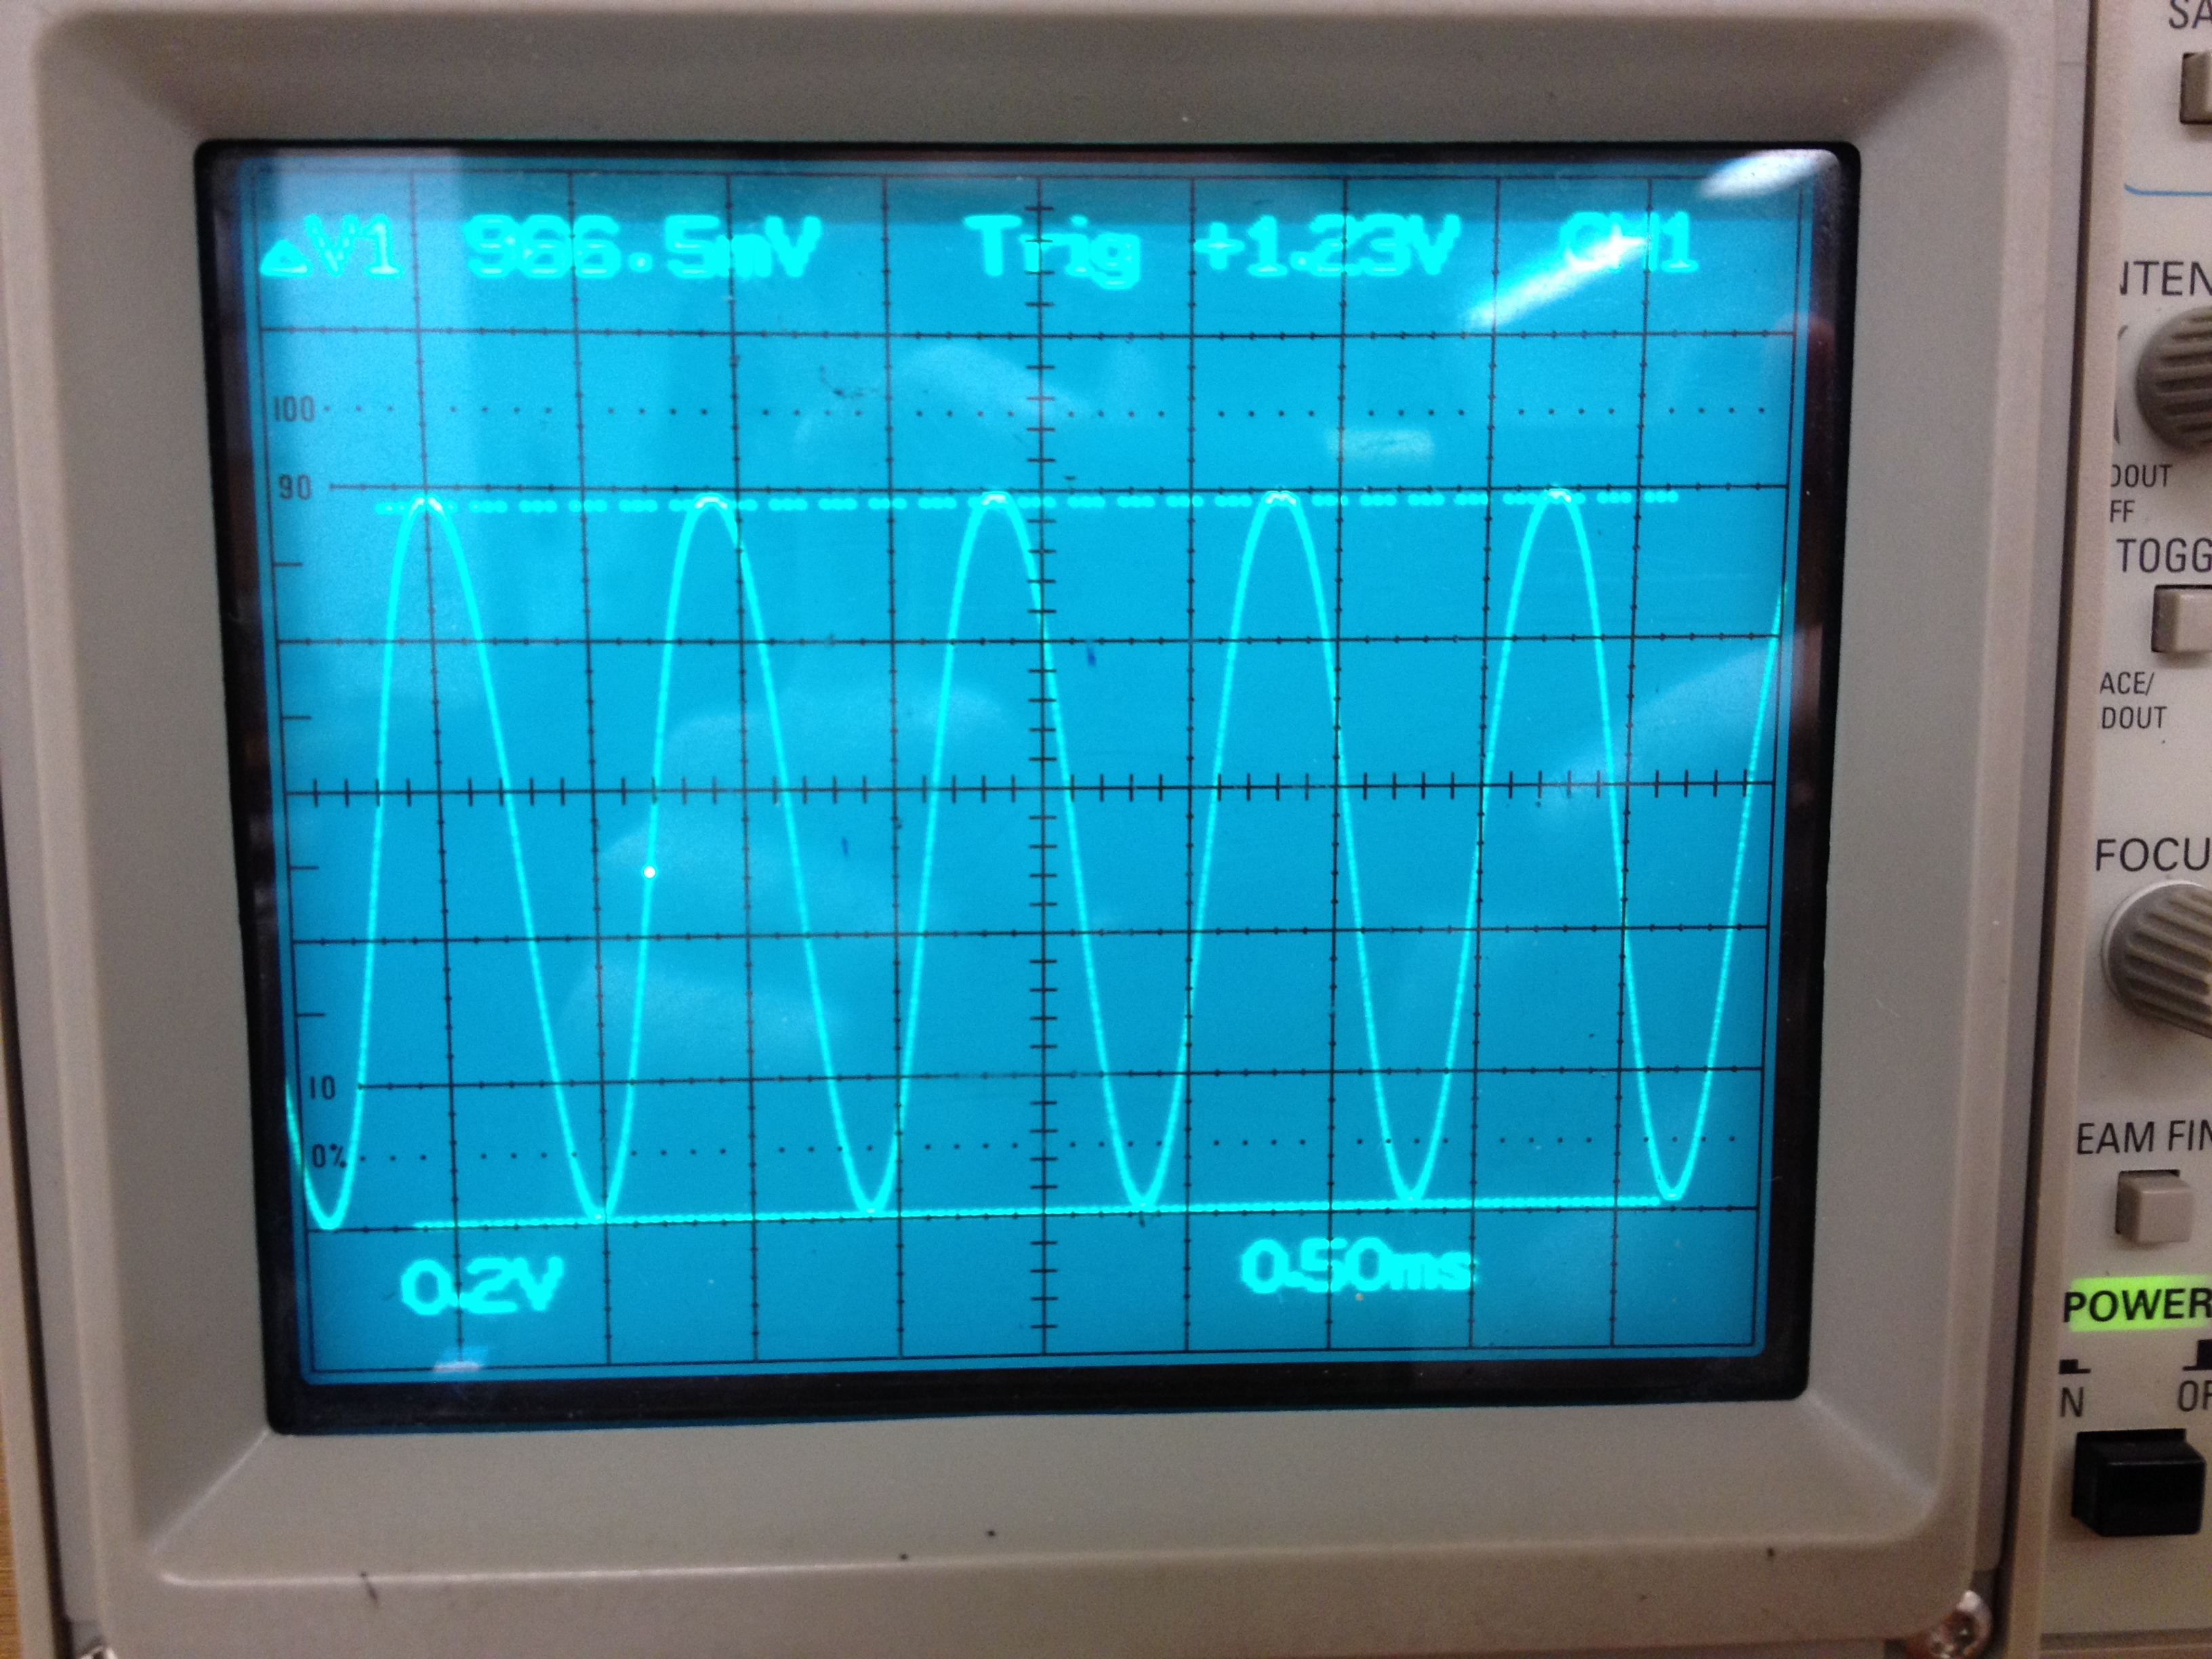
\includegraphics[width=\figwidth, keepaspectratio=true]{lab6_images/loading_output.jpg}
\caption{Output from Common Emitter Amplifier with input of 400 $mV_{pp}$ and emitter follower loading.}
\label{fig:loading_output}
\end{figure}

The measured component values for the emitter follower are $R_{E}$ = 982 $\Omega$ and $\beta$ = 243. Thus the expected voltage after the Common Emitter Amplifier is

$$
V_{CEA,closed} = 10.65 \frac{(1+243)982}{17670+(1+243)982} = 9.87 V.
$$

As shown in Figure \ref{fig:loading_output}, the measured voltage at that point was $V_{CEA,closed}$ = 9.67 $V_{pp}$, 2\% below the expected output.


\section*{Nonlinearity}
\subsection*{Procedure}
\begin{enumerate}
\item Increase the input amplitude until the output becomes nonlinear.
\end{enumerate}

\subsection*{Results}
\begin{figure}[H]
\centering
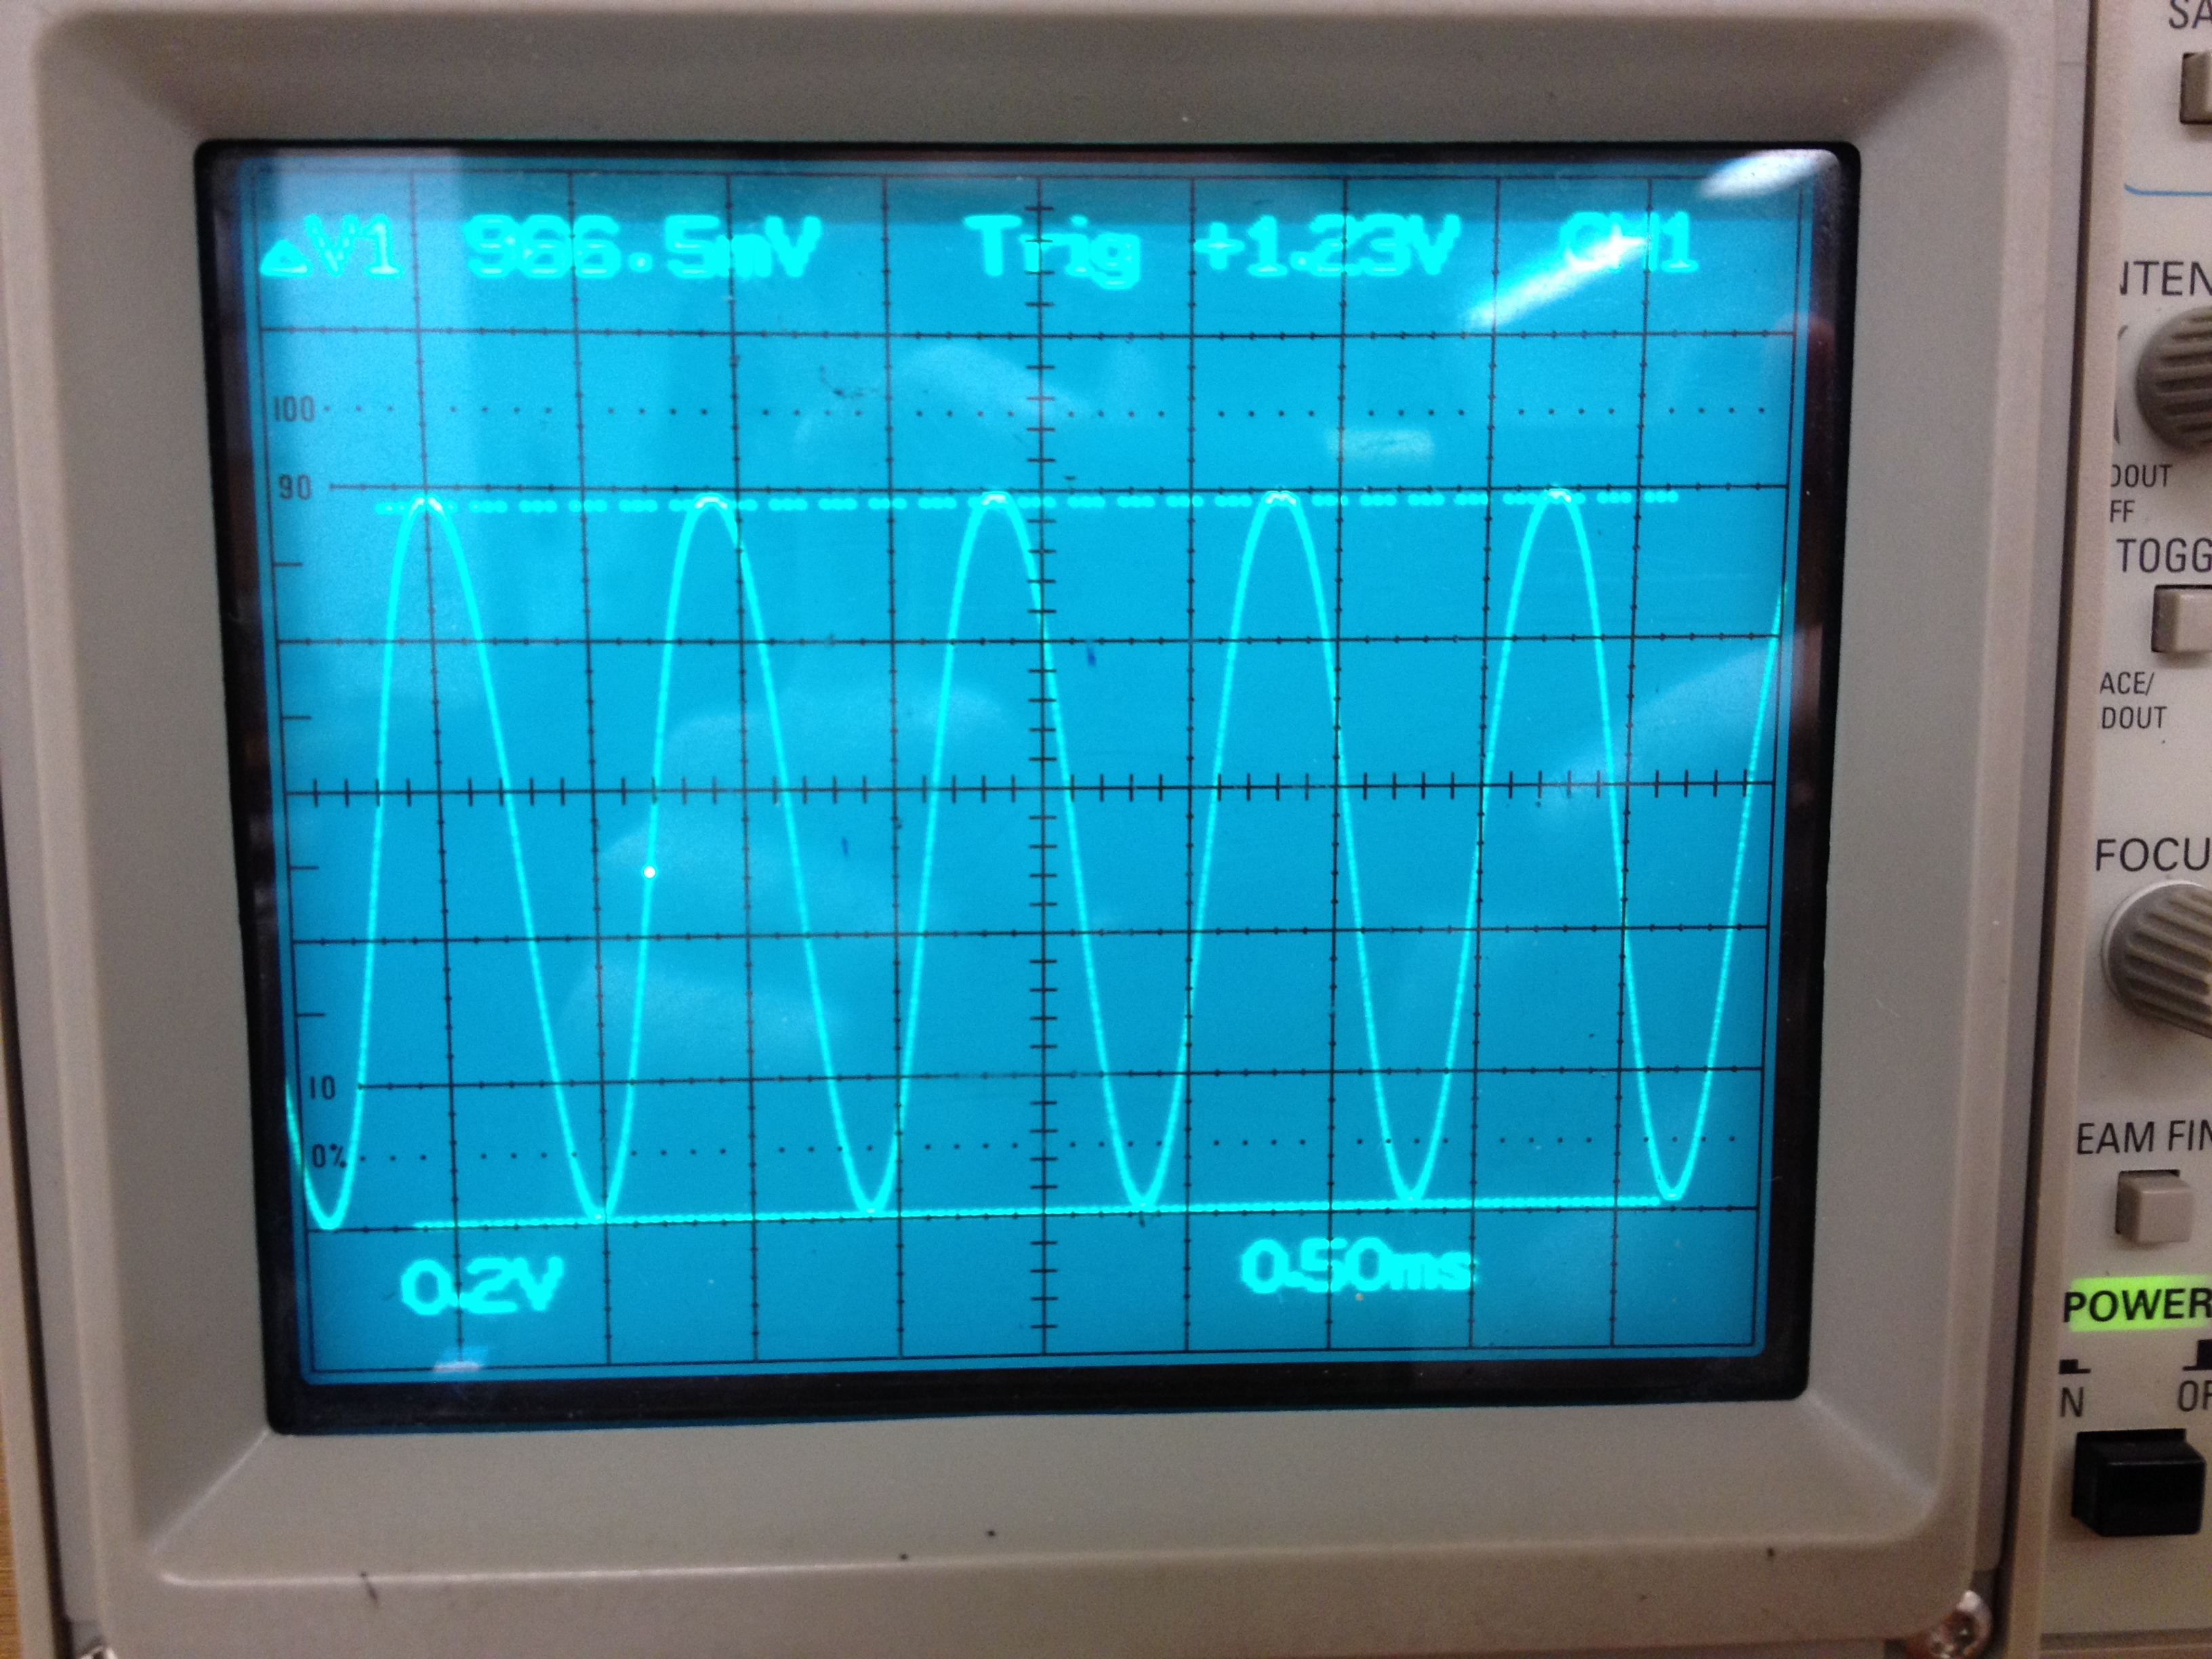
\includegraphics[width=\figwidth, keepaspectratio=true]{lab6_images/loading_output.jpg}
\caption{Output from Emitter Follower with input of 500 $mV_{pp}$.}
\label{fig:nonlinear_output}
\end{figure}

Increasing the input amplitude to 500 $mV_{pp}$ created the emitter follower output shown in \ref{fig:nonlinear_output} - clearly nonlinear. The output saturates very quickly as the input amplitude is increased because the emitter follower has no $R_C$. The lack of a collector resistor means the Q point voltage is high and already closer to the $V_{cc}$ value, meaning the transistor will reach saturation more easily than if there were an $R_C$.

\section*{Conclusion}
In conclusion, we observed what we expected for every section to with 6\%. We expected to see a drop in voltage gain when the emitter follower was added because it added a load to the output of the common emitter amplifier. The larger this load is, the smaller the drop is signal gain. We saw a drop from 10.65 V out to 9.67 V out, which corresponds well to the calculated expected value. The discrepancy of 0.2 V can be attributed to inaccuracy in measurements. Similarly, our unloaded output from the common emitter amplifier was within 6\% of expected magnitude. This lab has demonstrated the effects of loading and saturation when dealing with cascading transistor circuits.
\end{document}

%we see 6% less gain than expected by calculations because the DC bias is too high so there's clipping at the top of the sin wave. The positive portion of the sin wave gets to a lower amplitude than the negative portion
